\documentclass[twoside]{book}

% Packages required by doxygen
\usepackage{fixltx2e}
\usepackage{calc}
\usepackage{doxygen}
\usepackage[export]{adjustbox} % also loads graphicx
\usepackage{graphicx}
\usepackage[utf8]{inputenc}
\usepackage{makeidx}
\usepackage{multicol}
\usepackage{multirow}
\PassOptionsToPackage{warn}{textcomp}
\usepackage{textcomp}
\usepackage[nointegrals]{wasysym}
\usepackage[table]{xcolor}

% Font selection
\usepackage[T1]{fontenc}
\usepackage[scaled=.90]{helvet}
\usepackage{courier}
\usepackage{amssymb}
\usepackage{sectsty}
\renewcommand{\familydefault}{\sfdefault}
\allsectionsfont{%
  \fontseries{bc}\selectfont%
  \color{darkgray}%
}
\renewcommand{\DoxyLabelFont}{%
  \fontseries{bc}\selectfont%
  \color{darkgray}%
}
\newcommand{\+}{\discretionary{\mbox{\scriptsize$\hookleftarrow$}}{}{}}

% Page & text layout
\usepackage{geometry}
\geometry{%
  a4paper,%
  top=2.5cm,%
  bottom=2.5cm,%
  left=2.5cm,%
  right=2.5cm%
}
\tolerance=750
\hfuzz=15pt
\hbadness=750
\setlength{\emergencystretch}{15pt}
\setlength{\parindent}{0cm}
\setlength{\parskip}{3ex plus 2ex minus 2ex}
\makeatletter
\renewcommand{\paragraph}{%
  \@startsection{paragraph}{4}{0ex}{-1.0ex}{1.0ex}{%
    \normalfont\normalsize\bfseries\SS@parafont%
  }%
}
\renewcommand{\subparagraph}{%
  \@startsection{subparagraph}{5}{0ex}{-1.0ex}{1.0ex}{%
    \normalfont\normalsize\bfseries\SS@subparafont%
  }%
}
\makeatother

% Headers & footers
\usepackage{fancyhdr}
\pagestyle{fancyplain}
\fancyhead[LE]{\fancyplain{}{\bfseries\thepage}}
\fancyhead[CE]{\fancyplain{}{}}
\fancyhead[RE]{\fancyplain{}{\bfseries\leftmark}}
\fancyhead[LO]{\fancyplain{}{\bfseries\rightmark}}
\fancyhead[CO]{\fancyplain{}{}}
\fancyhead[RO]{\fancyplain{}{\bfseries\thepage}}
\fancyfoot[LE]{\fancyplain{}{}}
\fancyfoot[CE]{\fancyplain{}{}}
\fancyfoot[RE]{\fancyplain{}{\bfseries\scriptsize Generated by Doxygen }}
\fancyfoot[LO]{\fancyplain{}{\bfseries\scriptsize Generated by Doxygen }}
\fancyfoot[CO]{\fancyplain{}{}}
\fancyfoot[RO]{\fancyplain{}{}}
\renewcommand{\footrulewidth}{0.4pt}
\renewcommand{\chaptermark}[1]{%
  \markboth{#1}{}%
}
\renewcommand{\sectionmark}[1]{%
  \markright{\thesection\ #1}%
}

% Indices & bibliography
\usepackage{natbib}
\usepackage[titles]{tocloft}
\setcounter{tocdepth}{3}
\setcounter{secnumdepth}{5}
\makeindex

% Hyperlinks (required, but should be loaded last)
\usepackage{ifpdf}
\ifpdf
  \usepackage[pdftex,pagebackref=true]{hyperref}
\else
  \usepackage[ps2pdf,pagebackref=true]{hyperref}
\fi
\hypersetup{%
  colorlinks=true,%
  linkcolor=blue,%
  citecolor=blue,%
  unicode%
}

% Custom commands
\newcommand{\clearemptydoublepage}{%
  \newpage{\pagestyle{empty}\cleardoublepage}%
}

\usepackage{caption}
\captionsetup{labelsep=space,justification=centering,font={bf},singlelinecheck=off,skip=4pt,position=top}

%===== C O N T E N T S =====

\begin{document}

% Titlepage & ToC
\hypersetup{pageanchor=false,
             bookmarksnumbered=true,
             pdfencoding=unicode
            }
\pagenumbering{alph}
\begin{titlepage}
\vspace*{7cm}
\begin{center}%
{\Large Carto\+Pics \\[1ex]\large 1.\+0 }\\
\vspace*{1cm}
{\large Generated by Doxygen 1.8.13}\\
\end{center}
\end{titlepage}
\clearemptydoublepage
\pagenumbering{roman}
\tableofcontents
\clearemptydoublepage
\pagenumbering{arabic}
\hypersetup{pageanchor=true}

%--- Begin generated contents ---
\chapter{Carto\+Pics}
\label{md_README}
\Hypertarget{md_README}
Carto\+Pics is a simple script to generate Digital Elevation Model picture.

 ~\newline
 {\itshape Raster of a Brest\textquotesingle{}s harbour area} 

\subsection*{Getting Started}

These instructions will get you a copy of the project up and running on your local machine for development and testing purposes.

\subsubsection*{Prerequisites}

Let\textquotesingle{}s get started ! Clone the repository using git


\begin{DoxyCode}
git clone https://github.com/Teusner/CartoPics
\end{DoxyCode}


\subsubsection*{Compiling}

You are now able to compile the project


\begin{DoxyCode}
cd CartoPics/src
mkdir build
cd build
cmake ..
make
\end{DoxyCode}


create\+\_\+raster is now generate in Cartopics/src/build

\subsubsection*{First example}

To generate a Digital Elevation Model, you should have a file of the points you measured, as you can see on the following example


\begin{DoxyCode}
# latitude    longitude  elevation
48.29762887 -004.41737340 14.334
48.29762971 -004.41735997 14.379
48.29763698 -004.41738809 14.452
...
\end{DoxyCode}
 And then, run Carto\+Pics with the name of your file in parameter and the number of pixel along the x-\/axis


\begin{DoxyCode}
./cartopics my\_file.txt 1000
\end{DoxyCode}


You can find your output image in the same directory with the name {\itshape my\+\_\+file\+\_\+map.\+ppm}

\subsection*{Built With}


\begin{DoxyItemize}
\item \href{https://github.com/delfrrr/delaunator-cpp}{\tt delaunator-\/cpp} -\/ An efficient delaunay triangulation library
\item \href{https://github.com/richardroberts1992/Spectrum}{\tt Spectrum} -\/ A Color\+Map generator \href{http://cs.swan.ac.uk/~csbob/research/callCenter/color/roberts18spectrum.pdf}{\tt P\+DF Description}
\end{DoxyItemize}

\subsection*{Authors}


\begin{DoxyItemize}
\item {\bfseries Brateau Quentin} -\/ {\itshape Initial work} -\/ \href{https://github.com/Teusner}{\tt Teusner} \+:sunglasses\+:
\end{DoxyItemize}

\subsection*{License}

This project is licensed under the G\+NU General Public License v3.\+0 -\/ see the L\+I\+C\+E\+N\+SE.md file for details 
\chapter{Class Index}
\section{Class List}
Here are the classes, structs, unions and interfaces with brief descriptions\+:\begin{DoxyCompactList}
\item\contentsline{section}{\hyperlink{classCMList}{C\+M\+List} }{\pageref{classCMList}}{}
\item\contentsline{section}{\hyperlink{classColour}{Colour} }{\pageref{classColour}}{}
\item\contentsline{section}{\hyperlink{classColourManager}{Colour\+Manager} }{\pageref{classColourManager}}{}
\item\contentsline{section}{\hyperlink{classColourMap}{Colour\+Map} }{\pageref{classColourMap}}{}
\item\contentsline{section}{\hyperlink{structdelaunator_1_1compare}{delaunator\+::compare} }{\pageref{structdelaunator_1_1compare}}{}
\item\contentsline{section}{\hyperlink{classdelaunator_1_1Delaunator}{delaunator\+::\+Delaunator} }{\pageref{classdelaunator_1_1Delaunator}}{}
\item\contentsline{section}{\hyperlink{structdelaunator_1_1DelaunatorPoint}{delaunator\+::\+Delaunator\+Point} }{\pageref{structdelaunator_1_1DelaunatorPoint}}{}
\item\contentsline{section}{\hyperlink{classDEM}{D\+EM} \\*Digital Elevation Model }{\pageref{classDEM}}{}
\item\contentsline{section}{\hyperlink{classPixel}{Pixel} \\*\hyperlink{classPixel}{Pixel} for image processing }{\pageref{classPixel}}{}
\item\contentsline{section}{\hyperlink{classPoint}{Point} \\*\hyperlink{classPoint}{Point} representing for \hyperlink{classDEM}{D\+EM} }{\pageref{classPoint}}{}
\item\contentsline{section}{\hyperlink{structStats}{Stats} }{\pageref{structStats}}{}
\item\contentsline{section}{\hyperlink{classTriangle}{Triangle} \\*\hyperlink{classTriangle}{Triangle} for \hyperlink{classDEM}{D\+EM} }{\pageref{classTriangle}}{}
\end{DoxyCompactList}

\chapter{File Index}
\section{File List}
Here is a list of all documented files with brief descriptions\+:\begin{DoxyCompactList}
\item\contentsline{section}{include/{\bfseries colourmanager.\+h} }{\pageref{colourmanager_8h}}{}
\item\contentsline{section}{include/{\bfseries delaunator.\+hpp} }{\pageref{delaunator_8hpp}}{}
\item\contentsline{section}{include/\hyperlink{DEM_8hpp}{D\+E\+M.\+hpp} \\*\hyperlink{classDEM}{D\+EM} class for Digital Elevation model generating }{\pageref{DEM_8hpp}}{}
\item\contentsline{section}{include/{\bfseries Pixel.\+hpp} }{\pageref{Pixel_8hpp}}{}
\item\contentsline{section}{include/\hyperlink{tools_8hpp}{tools.\+hpp} \\*Tools for Digital Elevation model generating }{\pageref{tools_8hpp}}{}
\item\contentsline{section}{include/{\bfseries W\+G\+S84to\+Cartesian.\+hpp} }{\pageref{WGS84toCartesian_8hpp}}{}
\item\contentsline{section}{include/geometry/\hyperlink{Point_8hpp}{Point.\+hpp} \\*\hyperlink{classPoint}{Point} class }{\pageref{Point_8hpp}}{}
\item\contentsline{section}{include/geometry/\hyperlink{Triangle_8hpp}{Triangle.\+hpp} \\*\hyperlink{classTriangle}{Triangle} class for \hyperlink{classPixel}{Pixel} processing in Digital Elevation Model generating }{\pageref{Triangle_8hpp}}{}
\end{DoxyCompactList}

\chapter{Class Documentation}
\hypertarget{classCMList}{}\section{C\+M\+List Class Reference}
\label{classCMList}\index{C\+M\+List@{C\+M\+List}}


{\ttfamily \#include $<$colourmanager.\+h$>$}

\subsection*{Static Public Member Functions}
\begin{DoxyCompactItemize}
\item 
\mbox{\Hypertarget{classCMList_a80fd29892cd85578bb90ac0314d90fac}\label{classCMList_a80fd29892cd85578bb90ac0314d90fac}} 
static vector$<$ \hyperlink{classColourMap}{Colour\+Map} $>$ {\bfseries get\+Map\+List} (C\+M\+Classification cls=C\+M\+Classification\+::\+A\+NY)
\item 
\mbox{\Hypertarget{classCMList_a3625314068ac7105031ee21020987041}\label{classCMList_a3625314068ac7105031ee21020987041}} 
static void {\bfseries add\+Colour\+Map} (\hyperlink{classColourMap}{Colour\+Map} map)
\item 
\mbox{\Hypertarget{classCMList_a1b07fca77729021f4f8b0e9e20c964f6}\label{classCMList_a1b07fca77729021f4f8b0e9e20c964f6}} 
static vector$<$ \hyperlink{classColourMap}{Colour\+Map} $>$ \& {\bfseries return\+Complete\+Map\+List} ()
\item 
\mbox{\Hypertarget{classCMList_adfa7121839cd103ac76d2895a5a77065}\label{classCMList_adfa7121839cd103ac76d2895a5a77065}} 
static void {\bfseries setup\+Indexes\+In\+List} ()
\end{DoxyCompactItemize}


\subsection{Detailed Description}
The \hyperlink{classCMList}{C\+M\+List} holds a list of colour maps which the user can select from to set the currently used colour map. 

The documentation for this class was generated from the following file\+:\begin{DoxyCompactItemize}
\item 
include/colourmanager.\+h\end{DoxyCompactItemize}

\hypertarget{classColour}{}\section{Colour Class Reference}
\label{classColour}\index{Colour@{Colour}}


{\ttfamily \#include $<$colourmanager.\+h$>$}

\subsection*{Public Member Functions}
\begin{DoxyCompactItemize}
\item 
\mbox{\Hypertarget{classColour_a46612b9524fcd4cee818af6a86b7a4d2}\label{classColour_a46612b9524fcd4cee818af6a86b7a4d2}} 
\hyperlink{classColour_a46612b9524fcd4cee818af6a86b7a4d2}{Colour} ()
\begin{DoxyCompactList}\small\item\em An empty constructor for the class. $\ast$/. \end{DoxyCompactList}\item 
\hyperlink{classColour_a25a9ec348579c9df5363220ccbc1f3ec}{Colour} (float R, float G, float B, float A)
\begin{DoxyCompactList}\small\item\em A constructor for the \hyperlink{classColour}{Colour} class. \end{DoxyCompactList}\item 
\hyperlink{classColour_a4a447496ea54cc0d8b5f5cc5131ae0b6}{Colour} (float R, float G, float B, float A, std\+::string name)
\begin{DoxyCompactList}\small\item\em A constructor for the \hyperlink{classColour}{Colour} class. \end{DoxyCompactList}\item 
\hyperlink{classColour_a0a90c893db7eb92dd6fac4557123c3ac}{Colour} (std\+::string hex)
\begin{DoxyCompactList}\small\item\em A constructor for the \hyperlink{classColour}{Colour} class created using a colour hex value. \end{DoxyCompactList}\item 
std\+::string \hyperlink{classColour_a7f0220a8b5a1a0b476a1dc8f305484f7}{get\+Hex\+Colour} ()
\begin{DoxyCompactList}\small\item\em Returns the hex value of the colour object as a std\+::string. \end{DoxyCompactList}\item 
void \hyperlink{classColour_ade98ca5af3cde8f754e9b255dcaaeb24}{setR} (float R)
\begin{DoxyCompactList}\small\item\em Sets the red channel value. \end{DoxyCompactList}\item 
void \hyperlink{classColour_a7486867cf650aa822660cf40c394e06c}{setG} (float G)
\begin{DoxyCompactList}\small\item\em Sets the green channel value. \end{DoxyCompactList}\item 
void \hyperlink{classColour_ab29d4612841a580f2b668f1f2710b978}{setB} (float B)
\begin{DoxyCompactList}\small\item\em Sets the blue channel value. \end{DoxyCompactList}\item 
void \hyperlink{classColour_a894ca29ba370974e7e0be904ca9ba65e}{set\+Alpha} (float Alpha)
\begin{DoxyCompactList}\small\item\em Sets the colour alpha value. \end{DoxyCompactList}\item 
void \hyperlink{classColour_aeff40cb4f5ed87207c0efb2de32c01ad}{set\+Name\+ID} (std\+::string name)
\begin{DoxyCompactList}\small\item\em Sets the colour name. \end{DoxyCompactList}\item 
int \hyperlink{classColour_a3ac86075f6a02085c2d80c6648409f01}{get\+IntR} ()
\begin{DoxyCompactList}\small\item\em Gets the red channel value (0-\/255 int) \end{DoxyCompactList}\item 
int \hyperlink{classColour_a417a9c415589e6bb1163ca2e264ccb61}{get\+IntG} ()
\begin{DoxyCompactList}\small\item\em Gets the green channel value (0-\/255 int) \end{DoxyCompactList}\item 
int \hyperlink{classColour_a01d2ae35756ace52645d02be5ca001e0}{get\+IntB} ()
\begin{DoxyCompactList}\small\item\em Gets the blue channel value (0-\/255 int) \end{DoxyCompactList}\item 
float \hyperlink{classColour_a6237399e251d876aefe5d583ad251973}{getR} ()
\begin{DoxyCompactList}\small\item\em Gets the red channel value (0-\/1 float) \end{DoxyCompactList}\item 
float \hyperlink{classColour_aa16d7328c2acc3d701fd39593be50a65}{getG} ()
\begin{DoxyCompactList}\small\item\em Gets the green channel value (0-\/1 float) \end{DoxyCompactList}\item 
float \hyperlink{classColour_a9be696d70131487b8c2c4d92e09d5c8e}{getB} ()
\begin{DoxyCompactList}\small\item\em Gets the blue channel value (0-\/1 float) \end{DoxyCompactList}\item 
float \hyperlink{classColour_aa3108e4e8b6119a5e56222cd9e910219}{get\+Alpha} ()
\begin{DoxyCompactList}\small\item\em Gets the alpha channel value (0-\/1 float) \end{DoxyCompactList}\item 
std\+::string \hyperlink{classColour_a5f5329e70ac61e998658b4586ddfa753}{get\+Name\+ID} ()
\begin{DoxyCompactList}\small\item\em Gets the colour name. \end{DoxyCompactList}\end{DoxyCompactItemize}


\subsection{Detailed Description}
The \hyperlink{classColour}{Colour} class -\/ This holds the colour channel values and functions needed to produce R\+GB (float or int value) or hex values 

\subsection{Constructor \& Destructor Documentation}
\mbox{\Hypertarget{classColour_a25a9ec348579c9df5363220ccbc1f3ec}\label{classColour_a25a9ec348579c9df5363220ccbc1f3ec}} 
\index{Colour@{Colour}!Colour@{Colour}}
\index{Colour@{Colour}!Colour@{Colour}}
\subsubsection{\texorpdfstring{Colour()}{Colour()}\hspace{0.1cm}{\footnotesize\ttfamily [1/3]}}
{\footnotesize\ttfamily Colour\+::\+Colour (\begin{DoxyParamCaption}\item[{float}]{R,  }\item[{float}]{G,  }\item[{float}]{B,  }\item[{float}]{A }\end{DoxyParamCaption})\hspace{0.3cm}{\ttfamily [inline]}}



A constructor for the \hyperlink{classColour}{Colour} class. 


\begin{DoxyParams}{Parameters}
{\em R} & The red colour channel -\/ Either 0-\/1 OR 0-\/255 \\
\hline
{\em G} & The green colour channel -\/ Either 0-\/1 OR 0-\/255 \\
\hline
{\em B} & The blue colour channel -\/ Either 0-\/1 OR 0-\/255 \\
\hline
{\em A} & The alpha colour channel -\/ Either 0-\/1 OR 0-\/255 \\
\hline
\end{DoxyParams}
\mbox{\Hypertarget{classColour_a4a447496ea54cc0d8b5f5cc5131ae0b6}\label{classColour_a4a447496ea54cc0d8b5f5cc5131ae0b6}} 
\index{Colour@{Colour}!Colour@{Colour}}
\index{Colour@{Colour}!Colour@{Colour}}
\subsubsection{\texorpdfstring{Colour()}{Colour()}\hspace{0.1cm}{\footnotesize\ttfamily [2/3]}}
{\footnotesize\ttfamily Colour\+::\+Colour (\begin{DoxyParamCaption}\item[{float}]{R,  }\item[{float}]{G,  }\item[{float}]{B,  }\item[{float}]{A,  }\item[{std\+::string}]{name }\end{DoxyParamCaption})\hspace{0.3cm}{\ttfamily [inline]}}



A constructor for the \hyperlink{classColour}{Colour} class. 


\begin{DoxyParams}{Parameters}
{\em R} & The red colour channel -\/ float value either 0-\/1 OR 0-\/255 \\
\hline
{\em G} & The green colour channel -\/ float value Either 0-\/1 OR 0-\/255 \\
\hline
{\em B} & The blue colour channel -\/ float value Either 0-\/1 OR 0-\/255 \\
\hline
{\em A} & The alpha colour channel -\/ float value Either 0-\/1 OR 0-\/255 \\
\hline
{\em A} & The alpha colour channel -\/ float value Either 0-\/1 OR 0-\/255 \\
\hline
\end{DoxyParams}
\mbox{\Hypertarget{classColour_a0a90c893db7eb92dd6fac4557123c3ac}\label{classColour_a0a90c893db7eb92dd6fac4557123c3ac}} 
\index{Colour@{Colour}!Colour@{Colour}}
\index{Colour@{Colour}!Colour@{Colour}}
\subsubsection{\texorpdfstring{Colour()}{Colour()}\hspace{0.1cm}{\footnotesize\ttfamily [3/3]}}
{\footnotesize\ttfamily Colour\+::\+Colour (\begin{DoxyParamCaption}\item[{std\+::string}]{hex }\end{DoxyParamCaption})\hspace{0.3cm}{\ttfamily [inline]}}



A constructor for the \hyperlink{classColour}{Colour} class created using a colour hex value. 


\begin{DoxyParams}{Parameters}
{\em hex} & -\/ a string that contains the hex colour value. \\
\hline
\end{DoxyParams}


\subsection{Member Function Documentation}
\mbox{\Hypertarget{classColour_aa3108e4e8b6119a5e56222cd9e910219}\label{classColour_aa3108e4e8b6119a5e56222cd9e910219}} 
\index{Colour@{Colour}!get\+Alpha@{get\+Alpha}}
\index{get\+Alpha@{get\+Alpha}!Colour@{Colour}}
\subsubsection{\texorpdfstring{get\+Alpha()}{getAlpha()}}
{\footnotesize\ttfamily float Colour\+::get\+Alpha (\begin{DoxyParamCaption}{ }\end{DoxyParamCaption})\hspace{0.3cm}{\ttfamily [inline]}}



Gets the alpha channel value (0-\/1 float) 

\begin{DoxyReturn}{Returns}
float alpha channel value. 
\end{DoxyReturn}
\mbox{\Hypertarget{classColour_a9be696d70131487b8c2c4d92e09d5c8e}\label{classColour_a9be696d70131487b8c2c4d92e09d5c8e}} 
\index{Colour@{Colour}!getB@{getB}}
\index{getB@{getB}!Colour@{Colour}}
\subsubsection{\texorpdfstring{get\+B()}{getB()}}
{\footnotesize\ttfamily float Colour\+::getB (\begin{DoxyParamCaption}{ }\end{DoxyParamCaption})\hspace{0.3cm}{\ttfamily [inline]}}



Gets the blue channel value (0-\/1 float) 

\begin{DoxyReturn}{Returns}
float B channel value. 
\end{DoxyReturn}
\mbox{\Hypertarget{classColour_aa16d7328c2acc3d701fd39593be50a65}\label{classColour_aa16d7328c2acc3d701fd39593be50a65}} 
\index{Colour@{Colour}!getG@{getG}}
\index{getG@{getG}!Colour@{Colour}}
\subsubsection{\texorpdfstring{get\+G()}{getG()}}
{\footnotesize\ttfamily float Colour\+::getG (\begin{DoxyParamCaption}{ }\end{DoxyParamCaption})\hspace{0.3cm}{\ttfamily [inline]}}



Gets the green channel value (0-\/1 float) 

\begin{DoxyReturn}{Returns}
float G channel value. 
\end{DoxyReturn}
\mbox{\Hypertarget{classColour_a7f0220a8b5a1a0b476a1dc8f305484f7}\label{classColour_a7f0220a8b5a1a0b476a1dc8f305484f7}} 
\index{Colour@{Colour}!get\+Hex\+Colour@{get\+Hex\+Colour}}
\index{get\+Hex\+Colour@{get\+Hex\+Colour}!Colour@{Colour}}
\subsubsection{\texorpdfstring{get\+Hex\+Colour()}{getHexColour()}}
{\footnotesize\ttfamily std\+::string Colour\+::get\+Hex\+Colour (\begin{DoxyParamCaption}{ }\end{DoxyParamCaption})\hspace{0.3cm}{\ttfamily [inline]}}



Returns the hex value of the colour object as a std\+::string. 

\begin{DoxyReturn}{Returns}
std\+::string hex value 
\end{DoxyReturn}
\mbox{\Hypertarget{classColour_a01d2ae35756ace52645d02be5ca001e0}\label{classColour_a01d2ae35756ace52645d02be5ca001e0}} 
\index{Colour@{Colour}!get\+IntB@{get\+IntB}}
\index{get\+IntB@{get\+IntB}!Colour@{Colour}}
\subsubsection{\texorpdfstring{get\+Int\+B()}{getIntB()}}
{\footnotesize\ttfamily int Colour\+::get\+IntB (\begin{DoxyParamCaption}{ }\end{DoxyParamCaption})\hspace{0.3cm}{\ttfamily [inline]}}



Gets the blue channel value (0-\/255 int) 

\begin{DoxyReturn}{Returns}
int B channel value. 
\end{DoxyReturn}
\mbox{\Hypertarget{classColour_a417a9c415589e6bb1163ca2e264ccb61}\label{classColour_a417a9c415589e6bb1163ca2e264ccb61}} 
\index{Colour@{Colour}!get\+IntG@{get\+IntG}}
\index{get\+IntG@{get\+IntG}!Colour@{Colour}}
\subsubsection{\texorpdfstring{get\+Int\+G()}{getIntG()}}
{\footnotesize\ttfamily int Colour\+::get\+IntG (\begin{DoxyParamCaption}{ }\end{DoxyParamCaption})\hspace{0.3cm}{\ttfamily [inline]}}



Gets the green channel value (0-\/255 int) 

\begin{DoxyReturn}{Returns}
int B channel value. 
\end{DoxyReturn}
\mbox{\Hypertarget{classColour_a3ac86075f6a02085c2d80c6648409f01}\label{classColour_a3ac86075f6a02085c2d80c6648409f01}} 
\index{Colour@{Colour}!get\+IntR@{get\+IntR}}
\index{get\+IntR@{get\+IntR}!Colour@{Colour}}
\subsubsection{\texorpdfstring{get\+Int\+R()}{getIntR()}}
{\footnotesize\ttfamily int Colour\+::get\+IntR (\begin{DoxyParamCaption}{ }\end{DoxyParamCaption})\hspace{0.3cm}{\ttfamily [inline]}}



Gets the red channel value (0-\/255 int) 

\begin{DoxyReturn}{Returns}
int R channel value. 
\end{DoxyReturn}
\mbox{\Hypertarget{classColour_a5f5329e70ac61e998658b4586ddfa753}\label{classColour_a5f5329e70ac61e998658b4586ddfa753}} 
\index{Colour@{Colour}!get\+Name\+ID@{get\+Name\+ID}}
\index{get\+Name\+ID@{get\+Name\+ID}!Colour@{Colour}}
\subsubsection{\texorpdfstring{get\+Name\+I\+D()}{getNameID()}}
{\footnotesize\ttfamily std\+::string Colour\+::get\+Name\+ID (\begin{DoxyParamCaption}{ }\end{DoxyParamCaption})\hspace{0.3cm}{\ttfamily [inline]}}



Gets the colour name. 

\begin{DoxyReturn}{Returns}
std\+::string m\+\_\+\+Name\+ID name value; 
\end{DoxyReturn}
\mbox{\Hypertarget{classColour_a6237399e251d876aefe5d583ad251973}\label{classColour_a6237399e251d876aefe5d583ad251973}} 
\index{Colour@{Colour}!getR@{getR}}
\index{getR@{getR}!Colour@{Colour}}
\subsubsection{\texorpdfstring{get\+R()}{getR()}}
{\footnotesize\ttfamily float Colour\+::getR (\begin{DoxyParamCaption}{ }\end{DoxyParamCaption})\hspace{0.3cm}{\ttfamily [inline]}}



Gets the red channel value (0-\/1 float) 

\begin{DoxyReturn}{Returns}
float R channel value. 
\end{DoxyReturn}
\mbox{\Hypertarget{classColour_a894ca29ba370974e7e0be904ca9ba65e}\label{classColour_a894ca29ba370974e7e0be904ca9ba65e}} 
\index{Colour@{Colour}!set\+Alpha@{set\+Alpha}}
\index{set\+Alpha@{set\+Alpha}!Colour@{Colour}}
\subsubsection{\texorpdfstring{set\+Alpha()}{setAlpha()}}
{\footnotesize\ttfamily void Colour\+::set\+Alpha (\begin{DoxyParamCaption}\item[{float}]{Alpha }\end{DoxyParamCaption})\hspace{0.3cm}{\ttfamily [inline]}}



Sets the colour alpha value. 


\begin{DoxyParams}{Parameters}
{\em float} & Alpha -\/ the alpha value. \\
\hline
\end{DoxyParams}
\mbox{\Hypertarget{classColour_ab29d4612841a580f2b668f1f2710b978}\label{classColour_ab29d4612841a580f2b668f1f2710b978}} 
\index{Colour@{Colour}!setB@{setB}}
\index{setB@{setB}!Colour@{Colour}}
\subsubsection{\texorpdfstring{set\+B()}{setB()}}
{\footnotesize\ttfamily void Colour\+::setB (\begin{DoxyParamCaption}\item[{float}]{B }\end{DoxyParamCaption})\hspace{0.3cm}{\ttfamily [inline]}}



Sets the blue channel value. 


\begin{DoxyParams}{Parameters}
{\em float} & B -\/ the blue channel value. \\
\hline
\end{DoxyParams}
\mbox{\Hypertarget{classColour_a7486867cf650aa822660cf40c394e06c}\label{classColour_a7486867cf650aa822660cf40c394e06c}} 
\index{Colour@{Colour}!setG@{setG}}
\index{setG@{setG}!Colour@{Colour}}
\subsubsection{\texorpdfstring{set\+G()}{setG()}}
{\footnotesize\ttfamily void Colour\+::setG (\begin{DoxyParamCaption}\item[{float}]{G }\end{DoxyParamCaption})\hspace{0.3cm}{\ttfamily [inline]}}



Sets the green channel value. 


\begin{DoxyParams}{Parameters}
{\em float} & G -\/ the green channel value. \\
\hline
\end{DoxyParams}
\mbox{\Hypertarget{classColour_aeff40cb4f5ed87207c0efb2de32c01ad}\label{classColour_aeff40cb4f5ed87207c0efb2de32c01ad}} 
\index{Colour@{Colour}!set\+Name\+ID@{set\+Name\+ID}}
\index{set\+Name\+ID@{set\+Name\+ID}!Colour@{Colour}}
\subsubsection{\texorpdfstring{set\+Name\+I\+D()}{setNameID()}}
{\footnotesize\ttfamily void Colour\+::set\+Name\+ID (\begin{DoxyParamCaption}\item[{std\+::string}]{name }\end{DoxyParamCaption})\hspace{0.3cm}{\ttfamily [inline]}}



Sets the colour name. 


\begin{DoxyParams}{Parameters}
{\em std\+::string} & name -\/ the colour name. \\
\hline
\end{DoxyParams}
\mbox{\Hypertarget{classColour_ade98ca5af3cde8f754e9b255dcaaeb24}\label{classColour_ade98ca5af3cde8f754e9b255dcaaeb24}} 
\index{Colour@{Colour}!setR@{setR}}
\index{setR@{setR}!Colour@{Colour}}
\subsubsection{\texorpdfstring{set\+R()}{setR()}}
{\footnotesize\ttfamily void Colour\+::setR (\begin{DoxyParamCaption}\item[{float}]{R }\end{DoxyParamCaption})\hspace{0.3cm}{\ttfamily [inline]}}



Sets the red channel value. 


\begin{DoxyParams}{Parameters}
{\em float} & R -\/ the red channel value. \\
\hline
\end{DoxyParams}


The documentation for this class was generated from the following file\+:\begin{DoxyCompactItemize}
\item 
include/colourmanager.\+h\end{DoxyCompactItemize}

\hypertarget{classColourManager}{}\section{Colour\+Manager Class Reference}
\label{classColourManager}\index{Colour\+Manager@{Colour\+Manager}}


{\ttfamily \#include $<$colourmanager.\+h$>$}

\subsection*{Public Member Functions}
\begin{DoxyCompactItemize}
\item 
\mbox{\Hypertarget{classColourManager_af7e420271ffdb8aa1352be8f5c8d2c75}\label{classColourManager_af7e420271ffdb8aa1352be8f5c8d2c75}} 
float {\bfseries get\+Upper\+Range} ()
\item 
\mbox{\Hypertarget{classColourManager_ac9aacdcd5b240defc53e0273fb635501}\label{classColourManager_ac9aacdcd5b240defc53e0273fb635501}} 
void {\bfseries set\+Upper\+Range} (float Upper\+Range)
\item 
\mbox{\Hypertarget{classColourManager_a09c9c0da930b9fe390db80a19e5b96f9}\label{classColourManager_a09c9c0da930b9fe390db80a19e5b96f9}} 
float {\bfseries get\+Lower\+Range} ()
\item 
\mbox{\Hypertarget{classColourManager_a7555d13ef996799513a1cb1f29245f8d}\label{classColourManager_a7555d13ef996799513a1cb1f29245f8d}} 
void {\bfseries set\+Lower\+Range} (float Lower\+Range)
\item 
\mbox{\Hypertarget{classColourManager_a237206e41b8a7c81fe91ee477f9aeb9d}\label{classColourManager_a237206e41b8a7c81fe91ee477f9aeb9d}} 
\hyperlink{classColourMap}{Colour\+Map} \& {\bfseries get\+Current\+Colour\+Map} ()
\item 
\mbox{\Hypertarget{classColourManager_a846cefeecf0be6b441845ea9f8cb485c}\label{classColourManager_a846cefeecf0be6b441845ea9f8cb485c}} 
\hyperlink{classCMList}{C\+M\+List} \& {\bfseries get\+C\+M\+List} ()
\item 
\mbox{\Hypertarget{classColourManager_a316d945e07e2384cd34b5c502865466d}\label{classColourManager_a316d945e07e2384cd34b5c502865466d}} 
\hyperlink{classColour}{Colour} {\bfseries get\+Interpolated\+Colour} (float value)
\item 
\mbox{\Hypertarget{classColourManager_a1702cb7bf545735e9971c048612c3571}\label{classColourManager_a1702cb7bf545735e9971c048612c3571}} 
\hyperlink{classColour}{Colour} {\bfseries get\+Class\+Colour} (float value)
\item 
\mbox{\Hypertarget{classColourManager_a3d0b10403e8e035df59dc74ad9dadb0a}\label{classColourManager_a3d0b10403e8e035df59dc74ad9dadb0a}} 
\hyperlink{classColour}{Colour} {\bfseries get\+Colour\+From\+Seed} (uint seed)
\item 
\mbox{\Hypertarget{classColourManager_a1e97ddf97ab3794495007232466dc3a3}\label{classColourManager_a1e97ddf97ab3794495007232466dc3a3}} 
\hyperlink{classColour}{Colour} {\bfseries get\+Colour\+From\+Index} (int index)
\item 
\mbox{\Hypertarget{classColourManager_af17d269456ff97fd10a7a572b7aac7ec}\label{classColourManager_af17d269456ff97fd10a7a572b7aac7ec}} 
\hyperlink{classColour}{Colour} {\bfseries get\+Colour\+From\+Name} (std\+::string name)
\item 
\mbox{\Hypertarget{classColourManager_a52e3d1d62f621de0fe3e0868cdf280e9}\label{classColourManager_a52e3d1d62f621de0fe3e0868cdf280e9}} 
{\bfseries Colour\+Manager} (float lower\+Value, float upper\+Value)
\end{DoxyCompactItemize}
\subsection*{Static Public Member Functions}
\begin{DoxyCompactItemize}
\item 
\mbox{\Hypertarget{classColourManager_a77169e92057b8e4b7f8c17f69cc7c080}\label{classColourManager_a77169e92057b8e4b7f8c17f69cc7c080}} 
static int \& {\bfseries Colour\+Map\+Index} ()
\item 
\mbox{\Hypertarget{classColourManager_a073051c2f49306e7c4f64a4f8cb5d6c9}\label{classColourManager_a073051c2f49306e7c4f64a4f8cb5d6c9}} 
static void {\bfseries set\+Colour\+Map\+Index} (int index)
\item 
\mbox{\Hypertarget{classColourManager_a089f4867b6fad2d3fd89ee1165d32d5e}\label{classColourManager_a089f4867b6fad2d3fd89ee1165d32d5e}} 
static bool \& {\bfseries Invert\+Colour\+Map\+Flag} ()
\item 
\mbox{\Hypertarget{classColourManager_a9feb4edb18886847206e06e1724b97fc}\label{classColourManager_a9feb4edb18886847206e06e1724b97fc}} 
static void {\bfseries Invert\+Colour\+Map} ()
\item 
\mbox{\Hypertarget{classColourManager_ac92befd0cedb32c55e0b52ce76e0ac1e}\label{classColourManager_ac92befd0cedb32c55e0b52ce76e0ac1e}} 
static void {\bfseries set\+Current\+Colour\+Map} (\hyperlink{classColourMap}{Colour\+Map} \&map)
\item 
\mbox{\Hypertarget{classColourManager_af72400a23540302f29110fc2758e6adb}\label{classColourManager_af72400a23540302f29110fc2758e6adb}} 
static void {\bfseries Init\+\_\+\+Colour\+Manager} ()
\item 
\mbox{\Hypertarget{classColourManager_a1273e07cc4c45520937e7c60873a3832}\label{classColourManager_a1273e07cc4c45520937e7c60873a3832}} 
static void {\bfseries set\+Current\+Colour\+Map} ()
\item 
\mbox{\Hypertarget{classColourManager_af947b67fa4e61f4c5302beedcc730c8a}\label{classColourManager_af947b67fa4e61f4c5302beedcc730c8a}} 
static \hyperlink{classColourMap}{Colour\+Map} {\bfseries return\+Random\+Colour\+Map} (int seed=-\/1, int list\+Size=10)
\end{DoxyCompactItemize}


\subsection{Detailed Description}
The \hyperlink{classColourManager}{Colour\+Manager} class is the main manager for the colour maps. It handles the calculations of colour values and the current colour map. 

The documentation for this class was generated from the following file\+:\begin{DoxyCompactItemize}
\item 
include/colourmanager.\+h\end{DoxyCompactItemize}

\hypertarget{classColourMap}{}\section{Colour\+Map Class Reference}
\label{classColourMap}\index{Colour\+Map@{Colour\+Map}}


{\ttfamily \#include $<$colourmanager.\+h$>$}

\subsection*{Public Member Functions}
\begin{DoxyCompactItemize}
\item 
\mbox{\Hypertarget{classColourMap_a1a2a0c437c3f60d0f3d082387741d443}\label{classColourMap_a1a2a0c437c3f60d0f3d082387741d443}} 
{\bfseries Colour\+Map} (std\+::string name=\char`\"{}\char`\"{})
\item 
\mbox{\Hypertarget{classColourMap_ad378f3d48e33c2fb4d2214696b3ff276}\label{classColourMap_ad378f3d48e33c2fb4d2214696b3ff276}} 
void {\bfseries add\+Colour} (\hyperlink{classColour}{Colour} col)
\item 
\mbox{\Hypertarget{classColourMap_a6ce7c847e74160f0b5d5fa46ef7fe249}\label{classColourMap_a6ce7c847e74160f0b5d5fa46ef7fe249}} 
void {\bfseries add\+Colour} (float R, float G, float B, float F)
\item 
\mbox{\Hypertarget{classColourMap_a942403563c0a5b501fb1927187e2f3df}\label{classColourMap_a942403563c0a5b501fb1927187e2f3df}} 
void {\bfseries add\+Colour} (float R, float G, float B, float F, std\+::string name)
\item 
\mbox{\Hypertarget{classColourMap_a760a10f9844cd928c3404fee195cf502}\label{classColourMap_a760a10f9844cd928c3404fee195cf502}} 
\hyperlink{classColour}{Colour} \& {\bfseries operator\mbox{[}$\,$\mbox{]}} (const int i)
\item 
\mbox{\Hypertarget{classColourMap_a398cff20d5edad340b9794214d33c711}\label{classColourMap_a398cff20d5edad340b9794214d33c711}} 
\hyperlink{classColour}{Colour} {\bfseries operator\mbox{[}$\,$\mbox{]}} (const std\+::string name)
\item 
\mbox{\Hypertarget{classColourMap_a869eee79714568811b9bee1a61ebddc3}\label{classColourMap_a869eee79714568811b9bee1a61ebddc3}} 
const \hyperlink{classColour}{Colour} \& {\bfseries operator\mbox{[}$\,$\mbox{]}} (const int i) const
\item 
\mbox{\Hypertarget{classColourMap_aaf101d60702237a8c2d038f3b49ced66}\label{classColourMap_aaf101d60702237a8c2d038f3b49ced66}} 
vector$<$ \hyperlink{classColour}{Colour} $>$ \& {\bfseries get\+Colour\+List} ()
\item 
\mbox{\Hypertarget{classColourMap_ad32d03ad58020111e0d4699b0a4e597f}\label{classColourMap_ad32d03ad58020111e0d4699b0a4e597f}} 
const vector$<$ \hyperlink{classColour}{Colour} $>$ \& {\bfseries get\+Colour\+List} () const
\item 
\mbox{\Hypertarget{classColourMap_a08e9add60b5a7497166a8a7e5a0f860f}\label{classColourMap_a08e9add60b5a7497166a8a7e5a0f860f}} 
std\+::string {\bfseries get\+Map\+Name} ()
\item 
\mbox{\Hypertarget{classColourMap_aa8264cc2845d1253b8e8ede44be6e1c2}\label{classColourMap_aa8264cc2845d1253b8e8ede44be6e1c2}} 
int {\bfseries class\+Count} ()
\item 
\mbox{\Hypertarget{classColourMap_a0b1cfc5babfee416f8f2337712581eab}\label{classColourMap_a0b1cfc5babfee416f8f2337712581eab}} 
void {\bfseries set\+Map\+Name} (std\+::string name)
\item 
\mbox{\Hypertarget{classColourMap_a2802e6f099c8e224f7cb2d3d8dc3f4be}\label{classColourMap_a2802e6f099c8e224f7cb2d3d8dc3f4be}} 
C\+M\+Classification \& {\bfseries get\+Classification} ()
\item 
\mbox{\Hypertarget{classColourMap_a55bc63f784729b5ddda3180174842d29}\label{classColourMap_a55bc63f784729b5ddda3180174842d29}} 
void {\bfseries set\+Classification} (C\+M\+Classification cls)
\item 
\mbox{\Hypertarget{classColourMap_a4ef1038500ed24a5563cf0955d622e02}\label{classColourMap_a4ef1038500ed24a5563cf0955d622e02}} 
int {\bfseries get\+Index} ()
\item 
\mbox{\Hypertarget{classColourMap_a46ab3be1dc047c89f526d31e824f819e}\label{classColourMap_a46ab3be1dc047c89f526d31e824f819e}} 
void {\bfseries set\+Index} (int index)
\end{DoxyCompactItemize}


\subsection{Detailed Description}
This class holds a vector a colours which make up the colours of the colour map 

The documentation for this class was generated from the following file\+:\begin{DoxyCompactItemize}
\item 
include/colourmanager.\+h\end{DoxyCompactItemize}

\hypertarget{structdelaunator_1_1compare}{}\section{delaunator\+:\+:compare Struct Reference}
\label{structdelaunator_1_1compare}\index{delaunator\+::compare@{delaunator\+::compare}}
\subsection*{Public Member Functions}
\begin{DoxyCompactItemize}
\item 
\mbox{\Hypertarget{structdelaunator_1_1compare_a78b94657ec7bad085353f318365fa20a}\label{structdelaunator_1_1compare_a78b94657ec7bad085353f318365fa20a}} 
bool {\bfseries operator()} (std\+::size\+\_\+t i, std\+::size\+\_\+t j)
\end{DoxyCompactItemize}
\subsection*{Public Attributes}
\begin{DoxyCompactItemize}
\item 
\mbox{\Hypertarget{structdelaunator_1_1compare_a28fe3e7cd51ef236ac051fb47421321a}\label{structdelaunator_1_1compare_a28fe3e7cd51ef236ac051fb47421321a}} 
std\+::vector$<$ double $>$ const  \& {\bfseries coords}
\item 
\mbox{\Hypertarget{structdelaunator_1_1compare_a71238f2868c76ee8048cdd72d58da65c}\label{structdelaunator_1_1compare_a71238f2868c76ee8048cdd72d58da65c}} 
double {\bfseries cx}
\item 
\mbox{\Hypertarget{structdelaunator_1_1compare_ad8f7ce42823fff74a6062e439f93682d}\label{structdelaunator_1_1compare_ad8f7ce42823fff74a6062e439f93682d}} 
double {\bfseries cy}
\end{DoxyCompactItemize}


The documentation for this struct was generated from the following file\+:\begin{DoxyCompactItemize}
\item 
include/delaunator.\+hpp\end{DoxyCompactItemize}

\hypertarget{classdelaunator_1_1Delaunator}{}\section{delaunator\+:\+:Delaunator Class Reference}
\label{classdelaunator_1_1Delaunator}\index{delaunator\+::\+Delaunator@{delaunator\+::\+Delaunator}}
\subsection*{Public Member Functions}
\begin{DoxyCompactItemize}
\item 
\mbox{\Hypertarget{classdelaunator_1_1Delaunator_a094e288531f1695ca64437f0c04128c8}\label{classdelaunator_1_1Delaunator_a094e288531f1695ca64437f0c04128c8}} 
{\bfseries Delaunator} (std\+::vector$<$ double $>$ const \&in\+\_\+coords)
\item 
\mbox{\Hypertarget{classdelaunator_1_1Delaunator_ae6ee753d08679728afd4b603eab7d1ab}\label{classdelaunator_1_1Delaunator_ae6ee753d08679728afd4b603eab7d1ab}} 
double {\bfseries get\+\_\+hull\+\_\+area} ()
\end{DoxyCompactItemize}
\subsection*{Public Attributes}
\begin{DoxyCompactItemize}
\item 
\mbox{\Hypertarget{classdelaunator_1_1Delaunator_ac48ad29af151d66885120872bf46f750}\label{classdelaunator_1_1Delaunator_ac48ad29af151d66885120872bf46f750}} 
std\+::vector$<$ double $>$ const  \& {\bfseries coords}
\item 
\mbox{\Hypertarget{classdelaunator_1_1Delaunator_a6b613da33302f09aaea8fd74663d61cb}\label{classdelaunator_1_1Delaunator_a6b613da33302f09aaea8fd74663d61cb}} 
std\+::vector$<$ std\+::size\+\_\+t $>$ {\bfseries triangles}
\item 
\mbox{\Hypertarget{classdelaunator_1_1Delaunator_aff04629e1166358e4f2d43ed1e6524ef}\label{classdelaunator_1_1Delaunator_aff04629e1166358e4f2d43ed1e6524ef}} 
std\+::vector$<$ std\+::size\+\_\+t $>$ {\bfseries halfedges}
\item 
\mbox{\Hypertarget{classdelaunator_1_1Delaunator_a9d0f92cb1eee39f5ac80f65495d543c3}\label{classdelaunator_1_1Delaunator_a9d0f92cb1eee39f5ac80f65495d543c3}} 
std\+::vector$<$ std\+::size\+\_\+t $>$ {\bfseries hull\+\_\+prev}
\item 
\mbox{\Hypertarget{classdelaunator_1_1Delaunator_a8e6c50f7a0ff8c8b1f6e62c92004f57c}\label{classdelaunator_1_1Delaunator_a8e6c50f7a0ff8c8b1f6e62c92004f57c}} 
std\+::vector$<$ std\+::size\+\_\+t $>$ {\bfseries hull\+\_\+next}
\item 
\mbox{\Hypertarget{classdelaunator_1_1Delaunator_af9da27b2b5f8dc5b916b474078dd093a}\label{classdelaunator_1_1Delaunator_af9da27b2b5f8dc5b916b474078dd093a}} 
std\+::vector$<$ std\+::size\+\_\+t $>$ {\bfseries hull\+\_\+tri}
\item 
\mbox{\Hypertarget{classdelaunator_1_1Delaunator_a28717862d3ea8ae531ee2dc7fb57b639}\label{classdelaunator_1_1Delaunator_a28717862d3ea8ae531ee2dc7fb57b639}} 
std\+::size\+\_\+t {\bfseries hull\+\_\+start}
\end{DoxyCompactItemize}


The documentation for this class was generated from the following file\+:\begin{DoxyCompactItemize}
\item 
include/delaunator.\+hpp\end{DoxyCompactItemize}

\hypertarget{structdelaunator_1_1DelaunatorPoint}{}\section{delaunator\+:\+:Delaunator\+Point Struct Reference}
\label{structdelaunator_1_1DelaunatorPoint}\index{delaunator\+::\+Delaunator\+Point@{delaunator\+::\+Delaunator\+Point}}
\subsection*{Public Attributes}
\begin{DoxyCompactItemize}
\item 
\mbox{\Hypertarget{structdelaunator_1_1DelaunatorPoint_aa86be67d87cfc564557b05786ee0213b}\label{structdelaunator_1_1DelaunatorPoint_aa86be67d87cfc564557b05786ee0213b}} 
std\+::size\+\_\+t {\bfseries i}
\item 
\mbox{\Hypertarget{structdelaunator_1_1DelaunatorPoint_a6d0cf1b98a5ec895fcac5c1c2a10b926}\label{structdelaunator_1_1DelaunatorPoint_a6d0cf1b98a5ec895fcac5c1c2a10b926}} 
double {\bfseries x}
\item 
\mbox{\Hypertarget{structdelaunator_1_1DelaunatorPoint_a9137c3a0356dfc8a330b34f2944864a5}\label{structdelaunator_1_1DelaunatorPoint_a9137c3a0356dfc8a330b34f2944864a5}} 
double {\bfseries y}
\item 
\mbox{\Hypertarget{structdelaunator_1_1DelaunatorPoint_ab35213b07c403aa7ff3d927c7ca0d464}\label{structdelaunator_1_1DelaunatorPoint_ab35213b07c403aa7ff3d927c7ca0d464}} 
std\+::size\+\_\+t {\bfseries t}
\item 
\mbox{\Hypertarget{structdelaunator_1_1DelaunatorPoint_ab72027bce56e71be2d68440fbf261722}\label{structdelaunator_1_1DelaunatorPoint_ab72027bce56e71be2d68440fbf261722}} 
std\+::size\+\_\+t {\bfseries prev}
\item 
\mbox{\Hypertarget{structdelaunator_1_1DelaunatorPoint_aa6196f04bd176a2648d63f9235212f6b}\label{structdelaunator_1_1DelaunatorPoint_aa6196f04bd176a2648d63f9235212f6b}} 
std\+::size\+\_\+t {\bfseries next}
\item 
\mbox{\Hypertarget{structdelaunator_1_1DelaunatorPoint_ad2b84b88913a220615d6179ea6283b0d}\label{structdelaunator_1_1DelaunatorPoint_ad2b84b88913a220615d6179ea6283b0d}} 
bool {\bfseries removed}
\end{DoxyCompactItemize}


The documentation for this struct was generated from the following file\+:\begin{DoxyCompactItemize}
\item 
include/delaunator.\+hpp\end{DoxyCompactItemize}

\hypertarget{classDEM}{}\section{D\+EM Class Reference}
\label{classDEM}\index{D\+EM@{D\+EM}}


Digital Elevation Model.  




{\ttfamily \#include $<$D\+E\+M.\+hpp$>$}

\subsection*{Public Member Functions}
\begin{DoxyCompactItemize}
\item 
\hyperlink{classDEM_a64156558bc796710150012bf7873a2ad}{D\+EM} (const string \&ifname, const string \&ofname, const int \&x)
\begin{DoxyCompactList}\small\item\em Constructor. \end{DoxyCompactList}\item 
\hyperlink{classDEM_abd0e17d348572bcb75f94a23652828fc}{$\sim$\+D\+EM} ()
\begin{DoxyCompactList}\small\item\em Destructor. \end{DoxyCompactList}\item 
void \hyperlink{classDEM_aa335c6a15872db8075dcfc2074bc24a1}{read} (const string \&filename)
\begin{DoxyCompactList}\small\item\em read method \end{DoxyCompactList}\item 
void \hyperlink{classDEM_aadcc1b7e58d927d53d98356ad564ff30}{triangulation} (void)
\begin{DoxyCompactList}\small\item\em triangulation method \end{DoxyCompactList}\item 
void \hyperlink{classDEM_a1a9c426ce0626fea4f066b73c7045e6f}{process} (void)
\begin{DoxyCompactList}\small\item\em process method \end{DoxyCompactList}\item 
void \hyperlink{classDEM_ae5972d803d7f32e640fb732d4a98dfcf}{hill\+\_\+shading} (void)
\begin{DoxyCompactList}\small\item\em hill\+\_\+shading method \end{DoxyCompactList}\item 
void \hyperlink{classDEM_a6cb0c96b5a5b2d7c0f7ac07377a64dbd}{save} (string filename, int x, int y)
\begin{DoxyCompactList}\small\item\em save method \end{DoxyCompactList}\end{DoxyCompactItemize}
\subsection*{Public Attributes}
\begin{DoxyCompactItemize}
\item 
\mbox{\Hypertarget{classDEM_a22732c433a3cc1d4d8f9cb35e24395bc}\label{classDEM_a22732c433a3cc1d4d8f9cb35e24395bc}} 
double {\bfseries xmin}
\item 
\mbox{\Hypertarget{classDEM_a16f764fb785c33b98a8f011ed2bd8a43}\label{classDEM_a16f764fb785c33b98a8f011ed2bd8a43}} 
double {\bfseries xmax}
\item 
\mbox{\Hypertarget{classDEM_ad5dc7476428ed3f19d5007f7a7a1efd4}\label{classDEM_ad5dc7476428ed3f19d5007f7a7a1efd4}} 
double {\bfseries ymin}
\item 
\mbox{\Hypertarget{classDEM_a8e805974b711783d8e40fb9d1eda48a3}\label{classDEM_a8e805974b711783d8e40fb9d1eda48a3}} 
double {\bfseries ymax}
\item 
\mbox{\Hypertarget{classDEM_a9aaf109ccf41fedb0461de327e7d2945}\label{classDEM_a9aaf109ccf41fedb0461de327e7d2945}} 
double {\bfseries zmin}
\item 
\mbox{\Hypertarget{classDEM_a114f2350fe4801770ab19a213cb5674c}\label{classDEM_a114f2350fe4801770ab19a213cb5674c}} 
double {\bfseries zmax}
\item 
\mbox{\Hypertarget{classDEM_a666d01098888bbc8ad8fd8ef984c1f8b}\label{classDEM_a666d01098888bbc8ad8fd8ef984c1f8b}} 
float {\bfseries x\+\_\+labelizator} = 1
\item 
\mbox{\Hypertarget{classDEM_aec340951d2e311485b4e0e76a6c5161a}\label{classDEM_aec340951d2e311485b4e0e76a6c5161a}} 
float {\bfseries y\+\_\+labelizator} = 1
\end{DoxyCompactItemize}


\subsection{Detailed Description}
Digital Elevation Model. 

Let us create an object to load a file of cartographics data, and processing it to get a coloured image as an output. 

\subsection{Constructor \& Destructor Documentation}
\mbox{\Hypertarget{classDEM_a64156558bc796710150012bf7873a2ad}\label{classDEM_a64156558bc796710150012bf7873a2ad}} 
\index{D\+EM@{D\+EM}!D\+EM@{D\+EM}}
\index{D\+EM@{D\+EM}!D\+EM@{D\+EM}}
\subsubsection{\texorpdfstring{D\+E\+M()}{DEM()}}
{\footnotesize\ttfamily D\+E\+M\+::\+D\+EM (\begin{DoxyParamCaption}\item[{const string \&}]{ifname,  }\item[{const string \&}]{ofname,  }\item[{const int \&}]{x }\end{DoxyParamCaption})}



Constructor. 

Constructor of the \hyperlink{classDEM}{D\+EM} class. It let us initialize the name of the input file, the name of the output file and the number of pixels for the x-\/axis of the output image. \mbox{\Hypertarget{classDEM_abd0e17d348572bcb75f94a23652828fc}\label{classDEM_abd0e17d348572bcb75f94a23652828fc}} 
\index{D\+EM@{D\+EM}!````~D\+EM@{$\sim$\+D\+EM}}
\index{````~D\+EM@{$\sim$\+D\+EM}!D\+EM@{D\+EM}}
\subsubsection{\texorpdfstring{$\sim$\+D\+E\+M()}{~DEM()}}
{\footnotesize\ttfamily D\+E\+M\+::$\sim$\+D\+EM (\begin{DoxyParamCaption}{ }\end{DoxyParamCaption})}



Destructor. 

Destructor of the \hyperlink{classDEM}{D\+EM} class. Let us destruct the image dynamically allocated during the Digital Elevation Model processing. 

\subsection{Member Function Documentation}
\mbox{\Hypertarget{classDEM_ae5972d803d7f32e640fb732d4a98dfcf}\label{classDEM_ae5972d803d7f32e640fb732d4a98dfcf}} 
\index{D\+EM@{D\+EM}!hill\+\_\+shading@{hill\+\_\+shading}}
\index{hill\+\_\+shading@{hill\+\_\+shading}!D\+EM@{D\+EM}}
\subsubsection{\texorpdfstring{hill\+\_\+shading()}{hill\_shading()}}
{\footnotesize\ttfamily void D\+E\+M\+::hill\+\_\+shading (\begin{DoxyParamCaption}\item[{void}]{ }\end{DoxyParamCaption})}



hill\+\_\+shading method 

This method add shading on the image, using the hill shading method, to have a better output. \mbox{\Hypertarget{classDEM_a1a9c426ce0626fea4f066b73c7045e6f}\label{classDEM_a1a9c426ce0626fea4f066b73c7045e6f}} 
\index{D\+EM@{D\+EM}!process@{process}}
\index{process@{process}!D\+EM@{D\+EM}}
\subsubsection{\texorpdfstring{process()}{process()}}
{\footnotesize\ttfamily void D\+E\+M\+::process (\begin{DoxyParamCaption}\item[{void}]{ }\end{DoxyParamCaption})}



process method 

This method process each pixels of the output image. \mbox{\Hypertarget{classDEM_aa335c6a15872db8075dcfc2074bc24a1}\label{classDEM_aa335c6a15872db8075dcfc2074bc24a1}} 
\index{D\+EM@{D\+EM}!read@{read}}
\index{read@{read}!D\+EM@{D\+EM}}
\subsubsection{\texorpdfstring{read()}{read()}}
{\footnotesize\ttfamily void D\+E\+M\+::read (\begin{DoxyParamCaption}\item[{const string \&}]{filename }\end{DoxyParamCaption})}



read method 

This method let us read a file of elevation data for \hyperlink{classDEM}{D\+EM} generating.


\begin{DoxyParams}{Parameters}
{\em filename} & \+: the name of the input file \\
\hline
\end{DoxyParams}
\mbox{\Hypertarget{classDEM_a6cb0c96b5a5b2d7c0f7ac07377a64dbd}\label{classDEM_a6cb0c96b5a5b2d7c0f7ac07377a64dbd}} 
\index{D\+EM@{D\+EM}!save@{save}}
\index{save@{save}!D\+EM@{D\+EM}}
\subsubsection{\texorpdfstring{save()}{save()}}
{\footnotesize\ttfamily void D\+E\+M\+::save (\begin{DoxyParamCaption}\item[{string}]{filename,  }\item[{int}]{x,  }\item[{int}]{y }\end{DoxyParamCaption})}



save method 

This method let use save the created image. \mbox{\Hypertarget{classDEM_aadcc1b7e58d927d53d98356ad564ff30}\label{classDEM_aadcc1b7e58d927d53d98356ad564ff30}} 
\index{D\+EM@{D\+EM}!triangulation@{triangulation}}
\index{triangulation@{triangulation}!D\+EM@{D\+EM}}
\subsubsection{\texorpdfstring{triangulation()}{triangulation()}}
{\footnotesize\ttfamily void D\+E\+M\+::triangulation (\begin{DoxyParamCaption}\item[{void}]{ }\end{DoxyParamCaption})}



triangulation method 

This method set up a Delaunay\textquotesingle{}s triangulation on the data and labelize the triangles to make the search in these triangles easier. 

The documentation for this class was generated from the following files\+:\begin{DoxyCompactItemize}
\item 
include/\hyperlink{DEM_8hpp}{D\+E\+M.\+hpp}\item 
src/D\+E\+M.\+cpp\end{DoxyCompactItemize}

\hypertarget{classPixel}{}\section{Pixel Class Reference}
\label{classPixel}\index{Pixel@{Pixel}}


\hyperlink{classPixel}{Pixel} for image processing.  




{\ttfamily \#include $<$Pixel.\+hpp$>$}

\subsection*{Public Member Functions}
\begin{DoxyCompactItemize}
\item 
\hyperlink{classPixel_a27ad99a2f705e635c42d242d530d4756}{Pixel} ()
\begin{DoxyCompactList}\small\item\em Default constructor. \end{DoxyCompactList}\item 
void \hyperlink{classPixel_a8136f0a0bd54795ee065eeccb1e2ba1f}{set\+R\+GB} (float \&R, float \&G, float \&B)
\begin{DoxyCompactList}\small\item\em R\+GB Setter. \end{DoxyCompactList}\item 
void \hyperlink{classPixel_a992f88169f2395b752b5480f825efe72}{set\+H\+SV} (float \&H, float \&S, float \&V)
\begin{DoxyCompactList}\small\item\em H\+SV Setter. \end{DoxyCompactList}\item 
void \hyperlink{classPixel_a87c0f730000ab94e4d5bce5e2f4b435b}{get\+R\+GB} (float \&R, float \&G, float \&B)
\begin{DoxyCompactList}\small\item\em R\+GB Getter. \end{DoxyCompactList}\item 
void \hyperlink{classPixel_a70dc52435e31c139f3d04c601e2ca075}{get\+H\+SV} (float \&H, float \&S, float \&V)
\begin{DoxyCompactList}\small\item\em H\+SV Getter. \end{DoxyCompactList}\end{DoxyCompactItemize}
\subsection*{Friends}
\begin{DoxyCompactItemize}
\item 
std\+::ostream \& \hyperlink{classPixel_a3cbd62658db95c52ea5471707d3aaf01}{operator$<$$<$} (std\+::ostream \&stream, \hyperlink{classPixel}{Pixel} \&c)
\begin{DoxyCompactList}\small\item\em Stream operator $<$$<$. \end{DoxyCompactList}\end{DoxyCompactItemize}


\subsection{Detailed Description}
\hyperlink{classPixel}{Pixel} for image processing. 

This \hyperlink{classPixel}{Pixel} class let us set R\+GB and H\+SV values. You can use an array of \hyperlink{classPixel}{Pixel} to represent an image. 

\subsection{Constructor \& Destructor Documentation}
\mbox{\Hypertarget{classPixel_a27ad99a2f705e635c42d242d530d4756}\label{classPixel_a27ad99a2f705e635c42d242d530d4756}} 
\index{Pixel@{Pixel}!Pixel@{Pixel}}
\index{Pixel@{Pixel}!Pixel@{Pixel}}
\subsubsection{\texorpdfstring{Pixel()}{Pixel()}}
{\footnotesize\ttfamily Pixel\+::\+Pixel (\begin{DoxyParamCaption}{ }\end{DoxyParamCaption})}



Default constructor. 

Constructor of the \hyperlink{classPixel}{Pixel} class. 

\subsection{Member Function Documentation}
\mbox{\Hypertarget{classPixel_a70dc52435e31c139f3d04c601e2ca075}\label{classPixel_a70dc52435e31c139f3d04c601e2ca075}} 
\index{Pixel@{Pixel}!get\+H\+SV@{get\+H\+SV}}
\index{get\+H\+SV@{get\+H\+SV}!Pixel@{Pixel}}
\subsubsection{\texorpdfstring{get\+H\+S\+V()}{getHSV()}}
{\footnotesize\ttfamily void Pixel\+::get\+H\+SV (\begin{DoxyParamCaption}\item[{float \&}]{H,  }\item[{float \&}]{S,  }\item[{float \&}]{V }\end{DoxyParamCaption})}



H\+SV Getter. 

Getter for the coordinates of the \hyperlink{classPoint}{Point} class.


\begin{DoxyParams}{Parameters}
{\em H} & \+: getting the H value of the \hyperlink{classPixel}{Pixel} \\
\hline
{\em S} & \+: getting the S value of the \hyperlink{classPixel}{Pixel} \\
\hline
{\em V} & \+: getting the V value of the \hyperlink{classPixel}{Pixel} \\
\hline
\end{DoxyParams}
\mbox{\Hypertarget{classPixel_a87c0f730000ab94e4d5bce5e2f4b435b}\label{classPixel_a87c0f730000ab94e4d5bce5e2f4b435b}} 
\index{Pixel@{Pixel}!get\+R\+GB@{get\+R\+GB}}
\index{get\+R\+GB@{get\+R\+GB}!Pixel@{Pixel}}
\subsubsection{\texorpdfstring{get\+R\+G\+B()}{getRGB()}}
{\footnotesize\ttfamily void Pixel\+::get\+R\+GB (\begin{DoxyParamCaption}\item[{float \&}]{R,  }\item[{float \&}]{G,  }\item[{float \&}]{B }\end{DoxyParamCaption})}



R\+GB Getter. 

Getter for the coordinates of the \hyperlink{classPoint}{Point} class.


\begin{DoxyParams}{Parameters}
{\em R} & \+: getting the R value of the \hyperlink{classPixel}{Pixel} \\
\hline
{\em G} & \+: getting the G value of the \hyperlink{classPixel}{Pixel} \\
\hline
{\em B} & \+: getting the B value of the \hyperlink{classPixel}{Pixel} \\
\hline
\end{DoxyParams}
\mbox{\Hypertarget{classPixel_a992f88169f2395b752b5480f825efe72}\label{classPixel_a992f88169f2395b752b5480f825efe72}} 
\index{Pixel@{Pixel}!set\+H\+SV@{set\+H\+SV}}
\index{set\+H\+SV@{set\+H\+SV}!Pixel@{Pixel}}
\subsubsection{\texorpdfstring{set\+H\+S\+V()}{setHSV()}}
{\footnotesize\ttfamily void Pixel\+::set\+H\+SV (\begin{DoxyParamCaption}\item[{float \&}]{H,  }\item[{float \&}]{S,  }\item[{float \&}]{V }\end{DoxyParamCaption})}



H\+SV Setter. 

Setter for the coordinates of the \hyperlink{classPoint}{Point} class.


\begin{DoxyParams}{Parameters}
{\em H} & \+: newer H value for the \hyperlink{classPixel}{Pixel} \\
\hline
{\em S} & \+: newer S value for the \hyperlink{classPixel}{Pixel} \\
\hline
{\em V} & \+: newer V value for the \hyperlink{classPixel}{Pixel} \\
\hline
\end{DoxyParams}
\mbox{\Hypertarget{classPixel_a8136f0a0bd54795ee065eeccb1e2ba1f}\label{classPixel_a8136f0a0bd54795ee065eeccb1e2ba1f}} 
\index{Pixel@{Pixel}!set\+R\+GB@{set\+R\+GB}}
\index{set\+R\+GB@{set\+R\+GB}!Pixel@{Pixel}}
\subsubsection{\texorpdfstring{set\+R\+G\+B()}{setRGB()}}
{\footnotesize\ttfamily void Pixel\+::set\+R\+GB (\begin{DoxyParamCaption}\item[{float \&}]{R,  }\item[{float \&}]{G,  }\item[{float \&}]{B }\end{DoxyParamCaption})}



R\+GB Setter. 

Setter for the coordinates of the \hyperlink{classPoint}{Point} class.


\begin{DoxyParams}{Parameters}
{\em R} & \+: newer R value for the \hyperlink{classPixel}{Pixel} \\
\hline
{\em G} & \+: newer G value for the \hyperlink{classPixel}{Pixel} \\
\hline
{\em B} & \+: newer B value for the \hyperlink{classPixel}{Pixel} \\
\hline
\end{DoxyParams}


\subsection{Friends And Related Function Documentation}
\mbox{\Hypertarget{classPixel_a3cbd62658db95c52ea5471707d3aaf01}\label{classPixel_a3cbd62658db95c52ea5471707d3aaf01}} 
\index{Pixel@{Pixel}!operator$<$$<$@{operator$<$$<$}}
\index{operator$<$$<$@{operator$<$$<$}!Pixel@{Pixel}}
\subsubsection{\texorpdfstring{operator$<$$<$}{operator<<}}
{\footnotesize\ttfamily std\+::ostream\& operator$<$$<$ (\begin{DoxyParamCaption}\item[{std\+::ostream \&}]{stream,  }\item[{\hyperlink{classPixel}{Pixel} \&}]{c }\end{DoxyParamCaption})\hspace{0.3cm}{\ttfamily [friend]}}



Stream operator $<$$<$. 

To serialize the \hyperlink{classPixel}{Pixel} and easily save it to a file 

The documentation for this class was generated from the following files\+:\begin{DoxyCompactItemize}
\item 
include/Pixel.\+hpp\item 
src/Pixel.\+cpp\end{DoxyCompactItemize}

\hypertarget{classPoint}{}\section{Point Class Reference}
\label{classPoint}\index{Point@{Point}}


\hyperlink{classPoint}{Point} representing for \hyperlink{classDEM}{D\+EM}.  




{\ttfamily \#include $<$Point.\+hpp$>$}

\subsection*{Public Member Functions}
\begin{DoxyCompactItemize}
\item 
\hyperlink{classPoint_ad92f2337b839a94ce97dcdb439b4325a}{Point} ()
\begin{DoxyCompactList}\small\item\em Default Constructor. \end{DoxyCompactList}\item 
\hyperlink{classPoint_a4d43f5247afe8c85c6da1aa39dbcc738}{Point} (double x, double y, double z)
\begin{DoxyCompactList}\small\item\em Constructor. \end{DoxyCompactList}\item 
void \hyperlink{classPoint_a0100aa10290fdfc691e3fb0a6c8ed24a}{set\+Coords} (double x, double y, double z)
\begin{DoxyCompactList}\small\item\em Coords Setter. \end{DoxyCompactList}\end{DoxyCompactItemize}
\subsection*{Public Attributes}
\begin{DoxyCompactItemize}
\item 
\mbox{\Hypertarget{classPoint_a75a0d32cac6568a153e387789c020d37}\label{classPoint_a75a0d32cac6568a153e387789c020d37}} 
double {\bfseries m\+\_\+x}
\item 
\mbox{\Hypertarget{classPoint_a923b7de1d53753e6b3e927a30dd44286}\label{classPoint_a923b7de1d53753e6b3e927a30dd44286}} 
double {\bfseries m\+\_\+y}
\item 
\mbox{\Hypertarget{classPoint_a153a443818d11f43d48c1cefada558d9}\label{classPoint_a153a443818d11f43d48c1cefada558d9}} 
double {\bfseries m\+\_\+z}
\end{DoxyCompactItemize}


\subsection{Detailed Description}
\hyperlink{classPoint}{Point} representing for \hyperlink{classDEM}{D\+EM}. 

Let us create a \hyperlink{classPoint}{Point} object to facilitate data manipulation 

\subsection{Constructor \& Destructor Documentation}
\mbox{\Hypertarget{classPoint_ad92f2337b839a94ce97dcdb439b4325a}\label{classPoint_ad92f2337b839a94ce97dcdb439b4325a}} 
\index{Point@{Point}!Point@{Point}}
\index{Point@{Point}!Point@{Point}}
\subsubsection{\texorpdfstring{Point()}{Point()}\hspace{0.1cm}{\footnotesize\ttfamily [1/2]}}
{\footnotesize\ttfamily Point\+::\+Point (\begin{DoxyParamCaption}{ }\end{DoxyParamCaption})}



Default Constructor. 

Default constructor of the \hyperlink{classPoint}{Point} class. Each coordinate is set at 0.\+0. \mbox{\Hypertarget{classPoint_a4d43f5247afe8c85c6da1aa39dbcc738}\label{classPoint_a4d43f5247afe8c85c6da1aa39dbcc738}} 
\index{Point@{Point}!Point@{Point}}
\index{Point@{Point}!Point@{Point}}
\subsubsection{\texorpdfstring{Point()}{Point()}\hspace{0.1cm}{\footnotesize\ttfamily [2/2]}}
{\footnotesize\ttfamily Point\+::\+Point (\begin{DoxyParamCaption}\item[{double}]{x,  }\item[{double}]{y,  }\item[{double}]{z }\end{DoxyParamCaption})}



Constructor. 

Constructor of the \hyperlink{classPoint}{Point} class.


\begin{DoxyParams}{Parameters}
{\em x} & \+: x coordinate of the \hyperlink{classPoint}{Point} \\
\hline
{\em y} & \+: y coordinate of the \hyperlink{classPoint}{Point} \\
\hline
{\em z} & \+: z coordinate of the \hyperlink{classPoint}{Point} \\
\hline
\end{DoxyParams}


\subsection{Member Function Documentation}
\mbox{\Hypertarget{classPoint_a0100aa10290fdfc691e3fb0a6c8ed24a}\label{classPoint_a0100aa10290fdfc691e3fb0a6c8ed24a}} 
\index{Point@{Point}!set\+Coords@{set\+Coords}}
\index{set\+Coords@{set\+Coords}!Point@{Point}}
\subsubsection{\texorpdfstring{set\+Coords()}{setCoords()}}
{\footnotesize\ttfamily void Point\+::set\+Coords (\begin{DoxyParamCaption}\item[{double}]{x,  }\item[{double}]{y,  }\item[{double}]{z }\end{DoxyParamCaption})}



Coords Setter. 

Setter for the coordinates of the \hyperlink{classPoint}{Point} class.


\begin{DoxyParams}{Parameters}
{\em x} & \+: newer x coordinate of the \hyperlink{classPoint}{Point} \\
\hline
{\em y} & \+: newer y coordinate of the \hyperlink{classPoint}{Point} \\
\hline
{\em z} & \+: newer z coordinate of the \hyperlink{classPoint}{Point} \\
\hline
\end{DoxyParams}


The documentation for this class was generated from the following files\+:\begin{DoxyCompactItemize}
\item 
include/geometry/\hyperlink{Point_8hpp}{Point.\+hpp}\item 
src/Point.\+cpp\end{DoxyCompactItemize}

\hypertarget{structStats}{}\section{Stats Struct Reference}
\label{structStats}\index{Stats@{Stats}}
\subsection*{Public Attributes}
\begin{DoxyCompactItemize}
\item 
\mbox{\Hypertarget{structStats_a5ca5f37aa10d8f7ba2e36843fb0ff087}\label{structStats_a5ca5f37aa10d8f7ba2e36843fb0ff087}} 
double {\bfseries xmin}
\item 
\mbox{\Hypertarget{structStats_a453fb9f3707d50ac85dea73f2e98d44e}\label{structStats_a453fb9f3707d50ac85dea73f2e98d44e}} 
double {\bfseries xmax}
\item 
\mbox{\Hypertarget{structStats_aa51866119dad6edc67ed2925c1d6621b}\label{structStats_aa51866119dad6edc67ed2925c1d6621b}} 
double {\bfseries ymin}
\item 
\mbox{\Hypertarget{structStats_aff5d2ce3b5c29036904553625efab0be}\label{structStats_aff5d2ce3b5c29036904553625efab0be}} 
double {\bfseries ymax}
\item 
\mbox{\Hypertarget{structStats_a2b24842cc0de4a6be50dbb187bda7a6a}\label{structStats_a2b24842cc0de4a6be50dbb187bda7a6a}} 
double {\bfseries zmin}
\item 
\mbox{\Hypertarget{structStats_a01151cacd95b1d847e69aa92796be82a}\label{structStats_a01151cacd95b1d847e69aa92796be82a}} 
double {\bfseries zmax}
\end{DoxyCompactItemize}


The documentation for this struct was generated from the following file\+:\begin{DoxyCompactItemize}
\item 
include/\hyperlink{tools_8hpp}{tools.\+hpp}\end{DoxyCompactItemize}

\hypertarget{classTriangle}{}\section{Triangle Class Reference}
\label{classTriangle}\index{Triangle@{Triangle}}


\hyperlink{classTriangle}{Triangle} for \hyperlink{classDEM}{D\+EM}.  




{\ttfamily \#include $<$Triangle.\+hpp$>$}



Collaboration diagram for Triangle\+:
\nopagebreak
\begin{figure}[H]
\begin{center}
\leavevmode
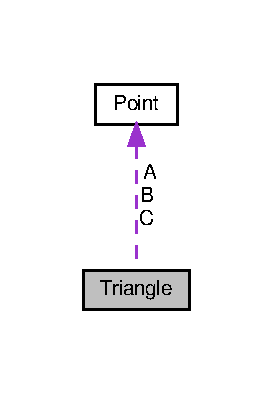
\includegraphics[width=131pt]{classTriangle__coll__graph}
\end{center}
\end{figure}
\subsection*{Public Member Functions}
\begin{DoxyCompactItemize}
\item 
\hyperlink{classTriangle_a3b15c4bcca06890db57e3a50d55ae7bb}{Triangle} (double xA, double yA, double zA, double xB, double yB, double zB, double xC, double yC, double zC)
\begin{DoxyCompactList}\small\item\em Constructor. \end{DoxyCompactList}\end{DoxyCompactItemize}
\subsection*{Public Attributes}
\begin{DoxyCompactItemize}
\item 
\mbox{\Hypertarget{classTriangle_a66edc1a5890531ea7550643c4866be59}\label{classTriangle_a66edc1a5890531ea7550643c4866be59}} 
\hyperlink{classPoint}{Point} {\bfseries A}
\item 
\mbox{\Hypertarget{classTriangle_a0e89c26ad3612019a8d3489c70c7d0e3}\label{classTriangle_a0e89c26ad3612019a8d3489c70c7d0e3}} 
\hyperlink{classPoint}{Point} {\bfseries B}
\item 
\mbox{\Hypertarget{classTriangle_ad5ef40fc843295b32ae0db058636d75e}\label{classTriangle_ad5ef40fc843295b32ae0db058636d75e}} 
\hyperlink{classPoint}{Point} {\bfseries C}
\item 
\mbox{\Hypertarget{classTriangle_a71c942f295b9fba50ab958ec29eeac7a}\label{classTriangle_a71c942f295b9fba50ab958ec29eeac7a}} 
double {\bfseries z}
\item 
\mbox{\Hypertarget{classTriangle_aaabd9fca950e2bb4ea08d47c360b1c4a}\label{classTriangle_aaabd9fca950e2bb4ea08d47c360b1c4a}} 
Eigen\+::\+Vector3d {\bfseries n}
\end{DoxyCompactItemize}


\subsection{Detailed Description}
\hyperlink{classTriangle}{Triangle} for \hyperlink{classDEM}{D\+EM}. 

\hyperlink{classTriangle}{Triangle} structure to process data during digital elevation model generating 

\subsection{Constructor \& Destructor Documentation}
\mbox{\Hypertarget{classTriangle_a3b15c4bcca06890db57e3a50d55ae7bb}\label{classTriangle_a3b15c4bcca06890db57e3a50d55ae7bb}} 
\index{Triangle@{Triangle}!Triangle@{Triangle}}
\index{Triangle@{Triangle}!Triangle@{Triangle}}
\subsubsection{\texorpdfstring{Triangle()}{Triangle()}}
{\footnotesize\ttfamily Triangle\+::\+Triangle (\begin{DoxyParamCaption}\item[{double}]{xA,  }\item[{double}]{yA,  }\item[{double}]{zA,  }\item[{double}]{xB,  }\item[{double}]{yB,  }\item[{double}]{zB,  }\item[{double}]{xC,  }\item[{double}]{yC,  }\item[{double}]{zC }\end{DoxyParamCaption})}



Constructor. 

Constructor of the \hyperlink{classTriangle}{Triangle} class.


\begin{DoxyParams}{Parameters}
{\em xA} & \+: x coordinate of the first point \\
\hline
{\em yA} & \+: y coordinate of the first point \\
\hline
{\em zA} & \+: x coordinate of the first point\\
\hline
{\em xB} & \+: x coordinate of the second point \\
\hline
{\em yB} & \+: y coordinate of the second point \\
\hline
{\em zB} & \+: x coordinate of the second point\\
\hline
{\em xC} & \+: x coordinate of the third point \\
\hline
{\em yC} & \+: y coordinate of the third point \\
\hline
{\em zC} & \+: x coordinate of the third point \\
\hline
\end{DoxyParams}


The documentation for this class was generated from the following files\+:\begin{DoxyCompactItemize}
\item 
include/geometry/\hyperlink{Triangle_8hpp}{Triangle.\+hpp}\item 
src/Triangle.\+cpp\end{DoxyCompactItemize}

\chapter{File Documentation}
\hypertarget{DEM_8hpp}{}\section{include/\+D\+EM.hpp File Reference}
\label{DEM_8hpp}\index{include/\+D\+E\+M.\+hpp@{include/\+D\+E\+M.\+hpp}}


\hyperlink{classDEM}{D\+EM} class for Digital Elevation model generating.  


{\ttfamily \#include $<$math.\+h$>$}\newline
{\ttfamily \#include $<$map$>$}\newline
{\ttfamily \#include $<$vector$>$}\newline
{\ttfamily \#include $<$iterator$>$}\newline
{\ttfamily \#include $<$iostream$>$}\newline
{\ttfamily \#include $<$iomanip$>$}\newline
{\ttfamily \#include $<$fstream$>$}\newline
{\ttfamily \#include $<$sstream$>$}\newline
{\ttfamily \#include $<$tools.\+hpp$>$}\newline
{\ttfamily \#include $<$Pixel.\+hpp$>$}\newline
{\ttfamily \#include $<$geometry/\+Triangle.\+hpp$>$}\newline
{\ttfamily \#include $<$geometry/\+Point.\+hpp$>$}\newline
Include dependency graph for D\+E\+M.\+hpp\+:
\nopagebreak
\begin{figure}[H]
\begin{center}
\leavevmode
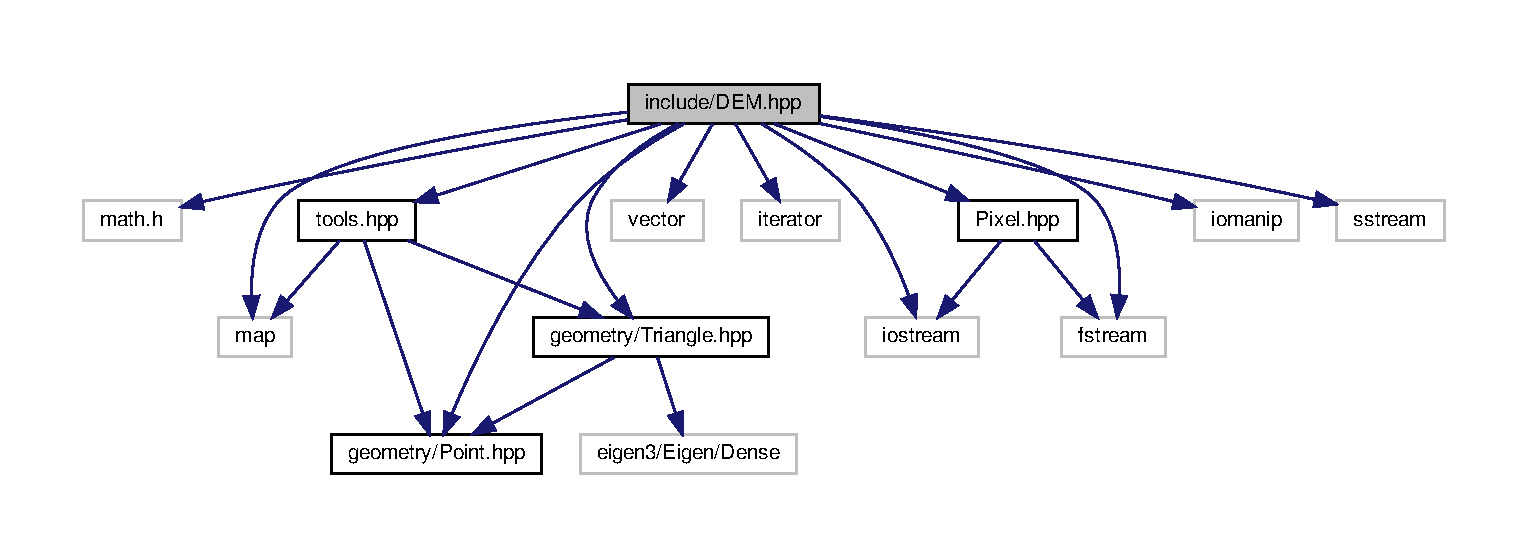
\includegraphics[width=350pt]{DEM_8hpp__incl}
\end{center}
\end{figure}
\subsection*{Classes}
\begin{DoxyCompactItemize}
\item 
class \hyperlink{classDEM}{D\+EM}
\begin{DoxyCompactList}\small\item\em Digital Elevation Model. \end{DoxyCompactList}\end{DoxyCompactItemize}


\subsection{Detailed Description}
\hyperlink{classDEM}{D\+EM} class for Digital Elevation model generating. 

\begin{DoxyAuthor}{Author}
brateaqu 
\end{DoxyAuthor}
\begin{DoxyVersion}{Version}
1.\+0 
\end{DoxyVersion}

\hypertarget{Point_8hpp}{}\section{include/geometry/\+Point.hpp File Reference}
\label{Point_8hpp}\index{include/geometry/\+Point.\+hpp@{include/geometry/\+Point.\+hpp}}


\hyperlink{classPoint}{Point} class.  


This graph shows which files directly or indirectly include this file\+:
\nopagebreak
\begin{figure}[H]
\begin{center}
\leavevmode
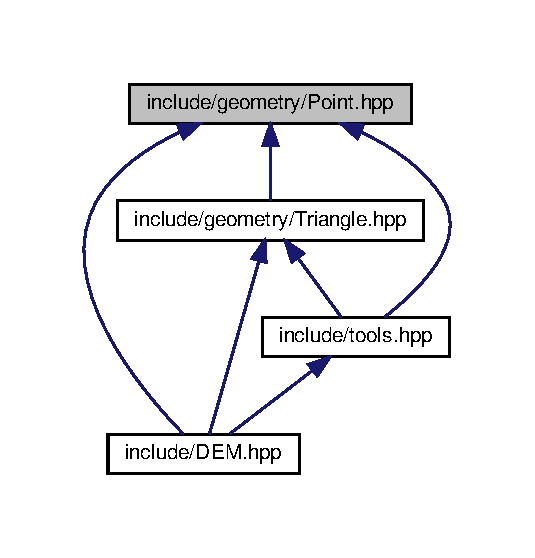
\includegraphics[width=257pt]{Point_8hpp__dep__incl}
\end{center}
\end{figure}
\subsection*{Classes}
\begin{DoxyCompactItemize}
\item 
class \hyperlink{classPoint}{Point}
\begin{DoxyCompactList}\small\item\em \hyperlink{classPoint}{Point} representing for \hyperlink{classDEM}{D\+EM}. \end{DoxyCompactList}\end{DoxyCompactItemize}


\subsection{Detailed Description}
\hyperlink{classPoint}{Point} class. 

\begin{DoxyAuthor}{Author}
brateaqu 
\end{DoxyAuthor}
\begin{DoxyVersion}{Version}
1.\+0 
\end{DoxyVersion}

\hypertarget{Triangle_8hpp}{}\section{include/geometry/\+Triangle.hpp File Reference}
\label{Triangle_8hpp}\index{include/geometry/\+Triangle.\+hpp@{include/geometry/\+Triangle.\+hpp}}


\hyperlink{classTriangle}{Triangle} class for \hyperlink{classPixel}{Pixel} processing in Digital Elevation Model generating.  


{\ttfamily \#include $<$eigen3/\+Eigen/\+Dense$>$}\newline
{\ttfamily \#include $<$geometry/\+Point.\+hpp$>$}\newline
Include dependency graph for Triangle.\+hpp\+:
\nopagebreak
\begin{figure}[H]
\begin{center}
\leavevmode
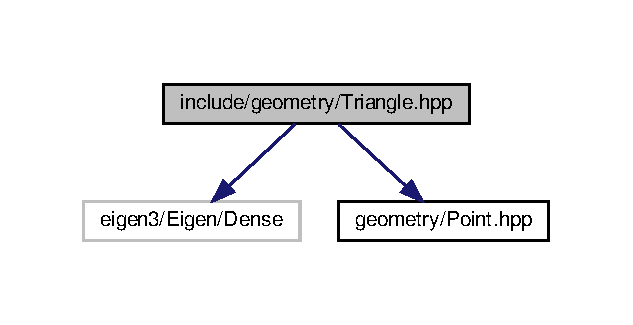
\includegraphics[width=304pt]{Triangle_8hpp__incl}
\end{center}
\end{figure}
This graph shows which files directly or indirectly include this file\+:\nopagebreak
\begin{figure}[H]
\begin{center}
\leavevmode
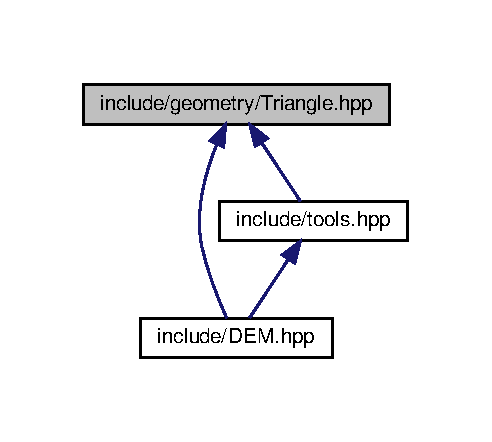
\includegraphics[width=236pt]{Triangle_8hpp__dep__incl}
\end{center}
\end{figure}
\subsection*{Classes}
\begin{DoxyCompactItemize}
\item 
class \hyperlink{classTriangle}{Triangle}
\begin{DoxyCompactList}\small\item\em \hyperlink{classTriangle}{Triangle} for \hyperlink{classDEM}{D\+EM}. \end{DoxyCompactList}\end{DoxyCompactItemize}


\subsection{Detailed Description}
\hyperlink{classTriangle}{Triangle} class for \hyperlink{classPixel}{Pixel} processing in Digital Elevation Model generating. 

\begin{DoxyAuthor}{Author}
brateaqu 
\end{DoxyAuthor}
\begin{DoxyVersion}{Version}
1.\+0 
\end{DoxyVersion}

\hypertarget{tools_8hpp}{}\section{include/tools.hpp File Reference}
\label{tools_8hpp}\index{include/tools.\+hpp@{include/tools.\+hpp}}


Tools for Digital Elevation model generating.  


{\ttfamily \#include $<$map$>$}\newline
{\ttfamily \#include $<$geometry/\+Triangle.\+hpp$>$}\newline
{\ttfamily \#include $<$geometry/\+Point.\+hpp$>$}\newline
Include dependency graph for tools.\+hpp\+:
\nopagebreak
\begin{figure}[H]
\begin{center}
\leavevmode
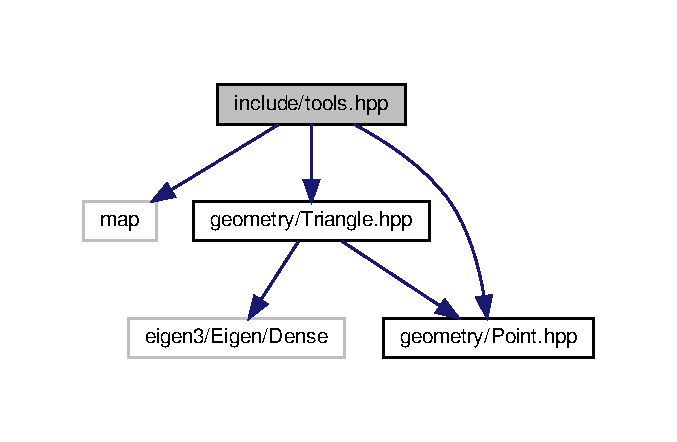
\includegraphics[width=325pt]{tools_8hpp__incl}
\end{center}
\end{figure}
This graph shows which files directly or indirectly include this file\+:\nopagebreak
\begin{figure}[H]
\begin{center}
\leavevmode
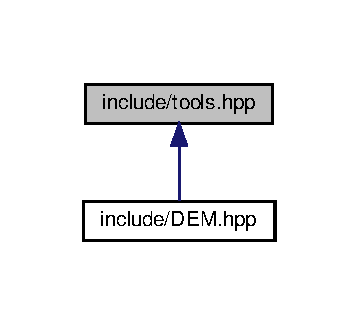
\includegraphics[width=172pt]{tools_8hpp__dep__incl}
\end{center}
\end{figure}
\subsection*{Classes}
\begin{DoxyCompactItemize}
\item 
struct \hyperlink{structStats}{Stats}
\end{DoxyCompactItemize}
\subsection*{Functions}
\begin{DoxyCompactItemize}
\item 
\hyperlink{structStats}{Stats} \hyperlink{tools_8hpp_afb19c04c1816c276612e24313cb2335a}{statistics} (std\+::map$<$ std\+::pair$<$ double, double $>$, double $>$ m\+\_\+map)
\begin{DoxyCompactList}\small\item\em statistics \end{DoxyCompactList}\item 
double \hyperlink{tools_8hpp_a0d1571de2c9f2667b12cb12131bc5e2b}{sign} (double P1x, double P1y, double P2x, double P2y, double P3x, double P3y)
\begin{DoxyCompactList}\small\item\em sign \end{DoxyCompactList}\item 
bool \hyperlink{tools_8hpp_acf041af12114025a246f9fa597aed1f3}{is\+Point\+In\+Triangle} (\hyperlink{classPoint}{Point} s, \hyperlink{classTriangle}{Triangle} T)
\begin{DoxyCompactList}\small\item\em is\+Point\+In\+Triangle \end{DoxyCompactList}\item 
bool \hyperlink{tools_8hpp_a250ba26e4ded1da8c46f34946d4d1e3a}{concave\+\_\+hull} (\hyperlink{classTriangle}{Triangle} T, float alpha)
\begin{DoxyCompactList}\small\item\em concave\+\_\+hull \end{DoxyCompactList}\end{DoxyCompactItemize}


\subsection{Detailed Description}
Tools for Digital Elevation model generating. 

\begin{DoxyAuthor}{Author}
brateaqu 
\end{DoxyAuthor}
\begin{DoxyVersion}{Version}
1.\+0 
\end{DoxyVersion}


\subsection{Function Documentation}
\mbox{\Hypertarget{tools_8hpp_a250ba26e4ded1da8c46f34946d4d1e3a}\label{tools_8hpp_a250ba26e4ded1da8c46f34946d4d1e3a}} 
\index{tools.\+hpp@{tools.\+hpp}!concave\+\_\+hull@{concave\+\_\+hull}}
\index{concave\+\_\+hull@{concave\+\_\+hull}!tools.\+hpp@{tools.\+hpp}}
\subsubsection{\texorpdfstring{concave\+\_\+hull()}{concave\_hull()}}
{\footnotesize\ttfamily bool concave\+\_\+hull (\begin{DoxyParamCaption}\item[{\hyperlink{classTriangle}{Triangle}}]{T,  }\item[{float}]{alpha }\end{DoxyParamCaption})}



concave\+\_\+hull 

This method help us to process a concave hull to the Delaunay\textquotesingle{}s triangulation data, which lead to create virtual triangles. Checking the restricted circle has a radius lower or equal at alpha.


\begin{DoxyParams}{Parameters}
{\em T} & \+: \hyperlink{classTriangle}{Triangle} object in which the \hyperlink{classPoint}{Point} should be. \\
\hline
{\em alpha} & \+: critical radius \\
\hline
\end{DoxyParams}
\mbox{\Hypertarget{tools_8hpp_acf041af12114025a246f9fa597aed1f3}\label{tools_8hpp_acf041af12114025a246f9fa597aed1f3}} 
\index{tools.\+hpp@{tools.\+hpp}!is\+Point\+In\+Triangle@{is\+Point\+In\+Triangle}}
\index{is\+Point\+In\+Triangle@{is\+Point\+In\+Triangle}!tools.\+hpp@{tools.\+hpp}}
\subsubsection{\texorpdfstring{is\+Point\+In\+Triangle()}{isPointInTriangle()}}
{\footnotesize\ttfamily bool is\+Point\+In\+Triangle (\begin{DoxyParamCaption}\item[{\hyperlink{classPoint}{Point}}]{s,  }\item[{\hyperlink{classTriangle}{Triangle}}]{T }\end{DoxyParamCaption})}



is\+Point\+In\+Triangle 

Checking if a \hyperlink{classPoint}{Point} is in a \hyperlink{classTriangle}{Triangle} for data processing in \hyperlink{classDEM}{D\+EM}.


\begin{DoxyParams}{Parameters}
{\em s} & \+: \hyperlink{classPoint}{Point} object \\
\hline
{\em T} & \+: \hyperlink{classTriangle}{Triangle} object in which the \hyperlink{classPoint}{Point} should be. \\
\hline
\end{DoxyParams}
\mbox{\Hypertarget{tools_8hpp_a0d1571de2c9f2667b12cb12131bc5e2b}\label{tools_8hpp_a0d1571de2c9f2667b12cb12131bc5e2b}} 
\index{tools.\+hpp@{tools.\+hpp}!sign@{sign}}
\index{sign@{sign}!tools.\+hpp@{tools.\+hpp}}
\subsubsection{\texorpdfstring{sign()}{sign()}}
{\footnotesize\ttfamily double sign (\begin{DoxyParamCaption}\item[{double}]{P1x,  }\item[{double}]{P1y,  }\item[{double}]{P2x,  }\item[{double}]{P2y,  }\item[{double}]{P3x,  }\item[{double}]{P3y }\end{DoxyParamCaption})}



sign 

Method used in is\+Point\+In\+Triangle. Determine the sign of a product


\begin{DoxyParams}{Parameters}
{\em P1\+\_\+x} & \+: x coordinate of the first point \\
\hline
{\em P1\+\_\+y} & \+: y coordinate of the first point \\
\hline
{\em P2\+\_\+x} & \+: x coordinate of the second point \\
\hline
{\em P2\+\_\+y} & \+: y coordinate of the second point \\
\hline
{\em P3\+\_\+x} & \+: x coordinate of the third point \\
\hline
{\em P3\+\_\+y} & \+: y coordinate of the third point \\
\hline
\end{DoxyParams}
\mbox{\Hypertarget{tools_8hpp_afb19c04c1816c276612e24313cb2335a}\label{tools_8hpp_afb19c04c1816c276612e24313cb2335a}} 
\index{tools.\+hpp@{tools.\+hpp}!statistics@{statistics}}
\index{statistics@{statistics}!tools.\+hpp@{tools.\+hpp}}
\subsubsection{\texorpdfstring{statistics()}{statistics()}}
{\footnotesize\ttfamily \hyperlink{structStats}{Stats} statistics (\begin{DoxyParamCaption}\item[{std\+::map$<$ std\+::pair$<$ double, double $>$, double $>$}]{m\+\_\+map }\end{DoxyParamCaption})}



statistics 

Processing statistics on a map. Extracting xmin, xmax, ymin, ymax, zmin and zmax on an map of pairs.


\begin{DoxyParams}{Parameters}
{\em m\+\_\+map} & \+: map of pairs of double \\
\hline
\end{DoxyParams}

%--- End generated contents ---

% Index
\backmatter
\newpage
\phantomsection
\clearemptydoublepage
\addcontentsline{toc}{chapter}{Index}
\printindex

\end{document}
